\documentclass[letterpaper]{article}

\usepackage{aaai}
\usepackage{amsmath}
\usepackage{amssymb}
\usepackage{amsthm}
\usepackage{courier}
\usepackage{graphicx}
\usepackage{helvet}
\usepackage{hyperref}
\usepackage{times}
\usepackage{verbatim}
\usepackage{wrapfig}

\newtheorem{definition}{Definition}
\newtheorem{example}{Example}
\newtheorem{formula}{Formula}
\newtheorem{problem}{Problem}

%\setlength\parindent{0pt}
\frenchspacing

\setlength{\pdfpagewidth}{8.5in}
\setlength{\pdfpageheight}{11in}

\pdfinfo{
/Title Pragmatic Semantics for the Web of Data
/Author Stefan Schlobach and Wouter Beek}
\setcounter{secnumdepth}{0}

\begin{document}

\title{Pragmatic Semantics for the Web of Data}
\author{Stefan Schlobach and Wouter Beek\\
Vrije Universiteit Amsterdam\\
De Boelelaan 1081a\\
1081HV Amsterdam\\
The Netherlands}
\maketitle
\begin{abstract}
\begin{quote}
The success of the Web of Data (WOD) is based on the thorough understanding of, and agreement upon, the semantics of data and ontologies. But the Web of Data as a whole is complex, and inherently messy, contextualised, opinionated, in short: it is a market-place of ideas, rather than a database. Existing paradigms are inappropriate for dealing with this new type of knowledge structures.

The urgency of dealing with the non-standard characteristics of the Web of Data has been recognised, and separate initiatives try to tackle its individual manifestations, e.g. inconsistencies, contexts, vagueness, provenance, etc. Tomorrow's Web of Data requires novel semantics with efficient (generic) implementations to ensure semantic clarity, reuse and interoperability.

We recently introduced pragmatic semantics  as a new semantic paradigm integrating elements from market theory and classical semantics into a framework of optimisation over truth-orderings, each representing a particular world-view. We propose nature-based algorithms to implement those semantics. We recently started a new research project, called PraSem, with the goal of investigating Pragmatic Semantics both from a theoretical and practical perspective.
\end{quote}
\end{abstract}

\section{Introduction}


 The Web of Data (WOD) connects data in a similar way as the WWW connects documents. Atomic data-units called resources are connected via typed links with arbitrary resources anywhere on the Web, and together these RDF triples form a gigantic graph of linked data. The meaning of the types can be fixed using standardised schema and ontology languages such as RDFS and OWL. The semantics of these languages are based on logical paradigms that were designed for small and hand-made knowledge bases, and come with a classical model-theory assigning truth to formulae, and entailment based on this truth. In a highly complex, dynamic, context-dependent, opinionated, contradictory and multi-dimensional semantic network as the WOD, these Semantics are insufficient, as they are one-dimensional, often prone to logical fallacies, and usually intractable.

Two simple scenarios will illustrate some of the high-level problems.

\begin{figure}[t]
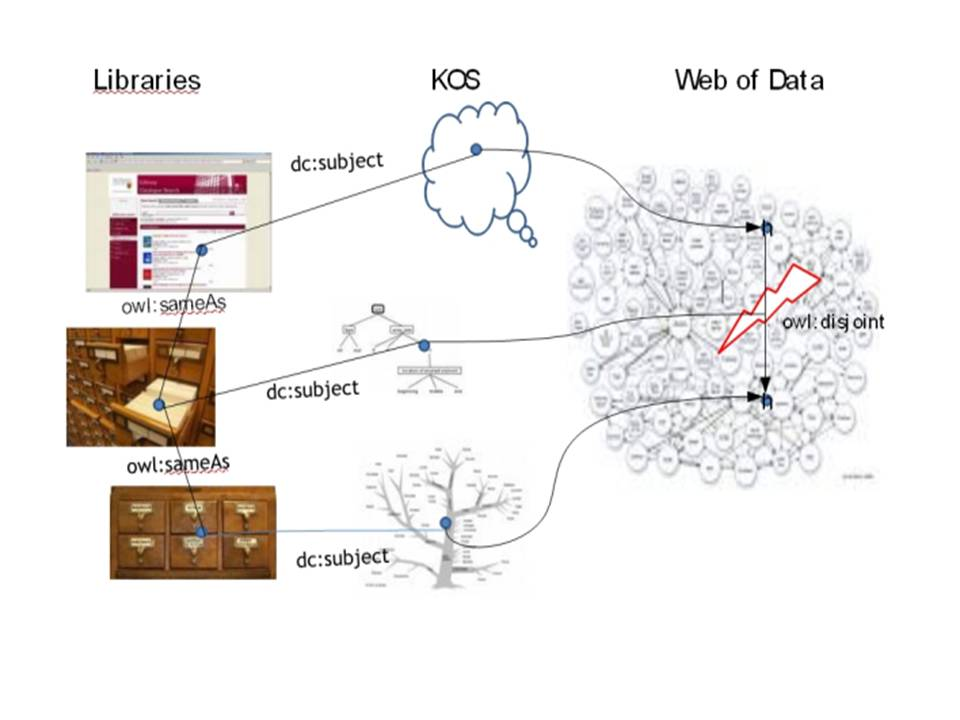
\includegraphics[width=\linewidth]{scenario1}
\caption{Scenario 1: heterogeneous publishing}
	\label{fig:ontograph}
\end{figure}

Scenario 1 is about heterogeneous publishing of data. Many libraries describe their books with controlled vocabularies. Linking collections and those vocabularies to the Linked-Open Data cloud, a collection of hundreds of interconnected data-graphs on the WOD, has huge benefits for libraries as search becomes more powerful, and metadata of documents is automatically enriched. Suppose a library in China annotates a book about Amsterdam with a concept ch:SmallTown. The Dutch National Library, on the other hand, annotates the same book with subject nl:BigCity. What happens now when the two libraries add their vocabularies and data to the WOD? What should be the desired answer to a query for big cities? Linking the libraries' vocabularies to the Linked-Open Data cloud will lead to conflicts and hamper access to the document in question rather than support it.

\begin{figure}[]
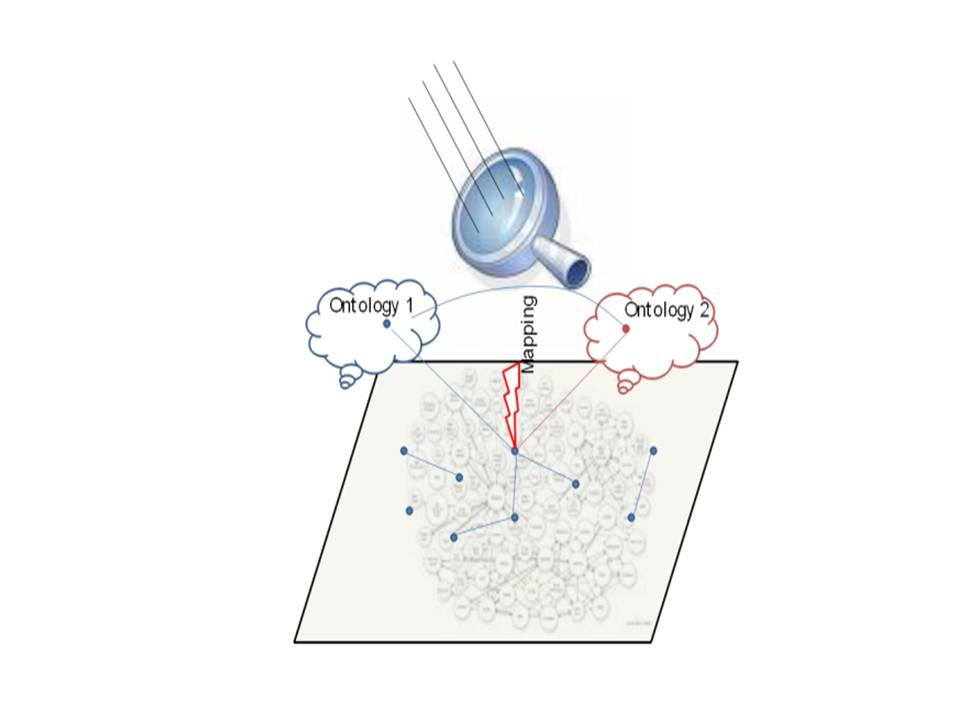
\includegraphics[width=\linewidth]{scenario2}
\caption{Scenario 2: opinionated data interpretation}
	\label{fig:ontograph}
\end{figure}


Scenario 2 is about opinionated interpretation of data, and is taken from Scientometrics, the Science of measuring and predicting Science. Scientometric researcher often use the Web as a proxy for studying science itself. Scientists leave online traces while doing research and a lot of this data is structured and part of the Web of Data. In some way, the WOD becomes a magnifying glass to measure activity in Science. The problem, however, is that multiple views are omnipresent: research blogs are biased, there are networks of publications of different impact levels, social networks that overshadow reliable analysis, which all comes on top of the usual technical problems of instance- unification, homonymy and synonymy. Modelling this highly complex Science Web with standard ontology languages is impossible as long as standard semantics are enforced.

On the Web in general, and the Web of Data in particular, almost every bit of information is context-dependent, biased towards a particular viewpoint, opinionated, dated, uncertain or vague. The WOD is a market-place of ideas, not a database, and has to be dealt with accordingly. As making the representational languages more complex is not an option, we have to adapt the formal semantics of existing formalisms to the new requirements.


\section{The need for a novel Semantic Paradigm}

The goal of our new research project, PraSem will be to introduce and assess the potential of novel semantics that can help overcome the weakness of traditional semantics when dealing with a messy, multi-dimensional, contextualised and complex knowledge structure such as the Web of Data.

\begin{figure}[t]
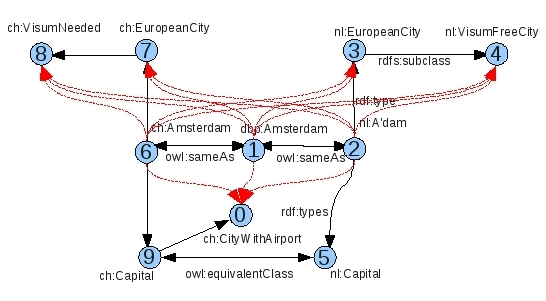
\includegraphics[width=\linewidth]{ontology_part}
\caption{An example ontology}
	\label{fig:ontograph}
\end{figure}

Consider a prototypical example: a Dutch dataset describes European cities, among them Amsterdam, which is a capital and does not require a visa for travel. In good practice the resources are linked to existing sources, e.g. DBpedia, by an owl:sameAs predicate. Similar data is published in China (using the namespace ch:), but now for European cities a visa is required. Both pieces of information are locally correct and the linking follows the correct principles. Still, considering the two classes ch:VisumNeeded and nl:VisumFreeCity to be disjoint, classical semantics collapse, and even useful derivable information, such as the fact that Amsterdam is a city with an airport, as it is a capital city, is lost. To address this issue, we need to deal with truth at different contexts.

Recent approaches to extend current methods, e.g., with quantitative information about vagueness and uncertainty, or towards multi-dimensionality are highly useful for specific applications. But they necessarily fall short of representing the full rich of the Web of Data. They also fail on a second, critical, requirement for our new semantics: as current ontology languages are already perceived as being too complex for practical use, the burden cannot be put on the modeller. We need to adapt the semantics, not the languages.

More concretely, we consider ontologies to be sets of RDF(S)/OWL triples. Without loss of generality an interpretation consists of a domain and interpretation function, assigning individuals to objects, concepts and classes to subsets of this domain, and properties and roles to binary relations, and which extended over the operators of the underlying representation language. Models are interpretations satisfying all the axioms. Axioms or triples are then classically entailed by the ontology if they are satisfied in all its models. Unfortunately, even in our simple example things go wrong as there cannot be a model where the instance dbp:Amsterdam is both visa-free and a city where a visa is required. By definition, everything is entailed: the semantics becomes useless.

\section{Pragmatic Semantics}

Pragmatic semantics integrate different world-views instead of defining meaning with respect to a single one. The idea is to make as much information in the data explicit, and turn it into first-class semantics citizens. First, it allows integrating classic model-theoretic notions of truth with explicit knowledge about the structure of the knowledge base. But also semantic meta-data, such as popularity, scarcity, abnormality, etc., and even background knowledge from other sources, can be integrated.

Most of this additional knowledge induces some kind of ordering on the formulas, which we will call truth orderings. A simple example of such a truth ordering is the one induced by the size of the minimal subontology classically entailing a formula. Other examples are orderings derived as the ratio of sub-models (models for parts of an ontology) in which a formula is satisfied versus the total number of sub-models, or the ratio between sub-ontologies of O in which a formula holds holds versus the number of all sub-ontologies are interesting candidates. Those are orderings based on subset of the ontology, a well-known class often used when dealing with inconsistent ontologies \cite{Huang}.

Another relevant class are orderings induced by the graph properties of the ontology, in case that the underlying data-model is graph-based. A shortest path ordering can be determined as the inverse of the longest shortest distance between all nodes in the ontology (diameter of the induced sub-graphs). Such a notion is a proxy for confidence of derivation. Other graph-based measures, e.g. based on random-walk distance or edge-weights, induce orderings that are clustering-aware; with sub-ontologies entailing a formula have more cohesion than others. Finally, taking node properties such as PageRank into account, orderings can be used as proxies for popularity.

While those two classes of orderings make structural properties of the ontology explicit and use them to implicitly contextualise meaning, others are based on external information outside the ontology itself. Examples for this are the Google count and similarity \cite{cilibrasi} based on frequency of labels of resources on the WWW.

The different orderings cover different aspects of the "true" semantics of the Web of Data. To combine those aspects pragmatic entailment is defined through multi-objective optimisation. A pragmatic closure C for an ontology O and orderings f1 to fn is then a set of formulas that is Pareto-optimal \cite{pareto} w.r.t. the optimisation problem $max\{f1 (C),�,fn (C)\}$.

Interoperability is then achieved by enriching an ontology with meta-information about semantic orderings, as well as agreement on the weighting of orderings. As there are possibly several pragmatic closures (different solutions on the Pareto-front) also agreement on the weighting of features is required. We will refer to the entailment induced by a given set of orderings as an instantiation of the family of pragmatic semantics.

\section{Calculi for Pragmatic Semantics}

Another way of looking at it is that the Web of Data is a Complex System \cite{gueretACS2011}, with interlinked information at different scales of abstraction. A well-argued claim in the Complex Systems literature suggests that it is impossible to construct logical systems that capture the full meaning of a true Complex System \cite{bar-yam}.

Results from studying the Web of Data as a Complex System show that considering different scales and levels of interactions make it impossible to engineer a web-scale reasoner (whatever the semantics considered), as traditional, decomposition-based approaches, are doomed with bandwidth limitations between the coordinating components (i.e. the datasets). Traditional semantics deal with this problem by an intrinsic reduction of the complexity: only one world-view, one perspective is considered at the time, the Web of Data is seen as a database. With pragmatic semantics, this advantage gets lost, and the computational price has to be paid, which applies that classical top-down reasoning becomes impossible.

It is often claimed that such systems have to evolve according to biological evolution rules \cite{36}, and web-scale semantics and reasoning should emerge from controlled interactions between autonomous components. In \cite{37} we introduced such a calculus based on swarm intelligence where instead of indexing all triples and joining the results, swarms of lightweight agents (so-called boids) autonomously traverse the graph, each representing a reasoning rule, which might be (partially) instantiated. Whenever the conditions of a rule match the node a boid is on, it locally adds the new derived triple. This provides an index-free alternative for reasoning over large distributed dynamic networks of RDF(S) graphs. It calculates the pragmatic closure under the condition of maximising popularity of nodes (as random walks of boids simulate PageRank calculation) and minimizing the length of sub-ontologies, two particular truth orderings. Not all of the conceivable calculi for pragmatic semantics have to be inspired by Computational Intelligence approaches, but PraSem will focus on this family of algorithms.

\section{Related Work}

The existing Semantic Web knowledge representation formalisms have been originally developed for describing crisp and static knowledge about a domain of application, and as such are essentially incapable of dealing with various contextual aspects of knowledge on the Web of Data, nor with a number of phenomena such as uncertainty, vagueness, ambiguity, which are a commonplace. On recognizing these limitations, much of the research effort of the Semantic Web community has been devoted to finding adequate ways of handling the newly identified tasks, resulting in a rich and heterogeneous body of work, e.g. on:
\begin{itemize}
\item	Reasoning with multiple ontologies, such as Integration and modularization, contextualisation and temporalisation. For the first e-Connections \cite{7,8} and Distributed Description Logics \cite{9} are typical examples. The extensive work on contextualization mostly provides extensions to DL and OWL-DL languages for representing contexts and context-dependent knowledge explicitly \cite{10,11,12} as does \cite{13} with temporalization.
\item	Reasoning with imperfect knowledge: non-standard extensions to the DL languages for representing uncertainty and vagueness, e.g. \cite{15,17}.
\item	Reasoning with multiple RDF graphs: extensions to the RDF framework based on formal aspects of multi-dimensionality, such as named graphs \cite{18}, networked graphs \cite{19} and multidimensional graphs \cite{20}. Also related: Ontology matching for semantic interoperability \cite{21,22,23} for some overviews, and more specifically for context dependency of matching \cite{24,25,26}).
\end{itemize}

Common to those approaches is their attempt to represent the complexity of the information explicitly, and as such put the burden on the shoulders of the user. All this work however indicates that devising semantics for this more complex and contextualised information is extremely hard, even when various aspects of the complexity are treated independently.

The most relevant attempt to introduce a new semantic paradigm has been Emergent Semantics \cite{27}, defining semantics as the result of collective processes and interactions between nodes in a network - a collective agreement. Although this formalism can capture some of the emerging structure, the price is that meaning and truth are defined as results of processes or calculi, and the well-understood declarative, model-theoretic semantics of traditional formalisms are lost. PraSem is orthogonal to emergent semantics: it can be seen as an attempt to explicitly capture as much semantic information as possible. For this, the semantic properties need to be captured in the truth functions, and the complexity be dealt within the optimisation process. For developing truth functions we will study the extensive literature on Complex Systems and graphs \cite{31,32}.

Very significant work on collective intelligence has proven to be effective for tasks such as network routing \cite{38} and data clustering \cite{39}, and using nature-inspired methods has become standard for optimization problems \cite{40,41}. They have also been investigate in the context of the Web of Data recently, such as for storage and querying \cite{42,orenISWC2008}, but to the best of our knowledge PraSem is novel in its attempt to use such methods as calculi for explicit semantic systems.

\bibliographystyle{aaai}
\bibliography{references}

\end{document}

